\documentclass[a4paper]{article}
\usepackage{graphicx}
\graphicspath{{./figures/}}
\usepackage[italian]{babel}
\usepackage{float}
\usepackage{braket}
\usepackage{listings}
\usepackage{mdframed}
\usepackage{tikz}
\usepackage{enumitem}
\usetikzlibrary{shapes, arrows, automata, petri, decorations.markings, decorations.pathreplacing, positioning, calc}

\usepackage{hyperref}
\hypersetup{
  colorlinks=false,
}

% Code blocks
\definecolor{codegreen}{rgb}{0,0.6,0}
\definecolor{codegray}{rgb}{0.5,0.5,0.5}
\definecolor{codepurple}{rgb}{0.58,0,0.82}
\definecolor{backcolour}{rgb}{0.95,0.95,0.95}

\lstdefinestyle{mystyle}{
  backgroundcolor=\color{backcolour},
  commentstyle=\color{codegreen},
  keywordstyle=\color{magenta},
  numberstyle=\tiny\color{codegray},
  stringstyle=\color{codepurple},
  basicstyle=\ttfamily\footnotesize,
  breakatwhitespace=false,
  breaklines=true,
  captionpos=b,
  keepspaces=true,
  numbers=left,
  numbersep=5pt,
  showspaces=false,
  showstringspaces=false,
  showtabs=false,
  tabsize=2
}

\lstset{style=mystyle}

\begin{document}

% Title ------------------------------------------------------------------------------
\title{Documentazione progetto Ingegneria del Software\\[1ex]
  \large Software di gestione dei pazienti diabetici
}

\author{
  \vspace{0.8cm}
  Università di Verona\\
  Imbriani Paolo - VR500437\\
  Irimie Fabio - VR501504
}

\begin{figure}
  \centering
  
\includegraphics[width=0.3\textwidth]{UniversityofVerona}
\end{figure}

\maketitle 

\pagebreak
% Title ------------------------------------------------------------------------------

\tableofcontents

\pagebreak

\section{Requisiti e Use Case}

\subsection{Note generali}

Il software che si andrà a sviluppare è un sistema di telemedicina di un servizio clinico per la gestione
di pazienti diabetici. Gli attori principali del sistema sono i \textit{medici} (diabetologi) e i \textit{pazienti}; questi ultimi
hanno credenziali di accesso al sistema fornite dagli amministratori del servizio con cui possono autenticarsi.
Se l'autenticazione va a buon fine allora l'utente verrà indirizzato alla propria \textit{home page} in cui potrà
visualizzare le informazioni relative al loro ruolo. Nel seguente diagramma dei casi d'uso sono rappresentati
i principali attori e le loro interazioni con il sistema. Notare che diamo per scontato che tutti gli autori siano già autenticati
per semplificare il diagramma.

\begin{figure}[H]
  \centering
  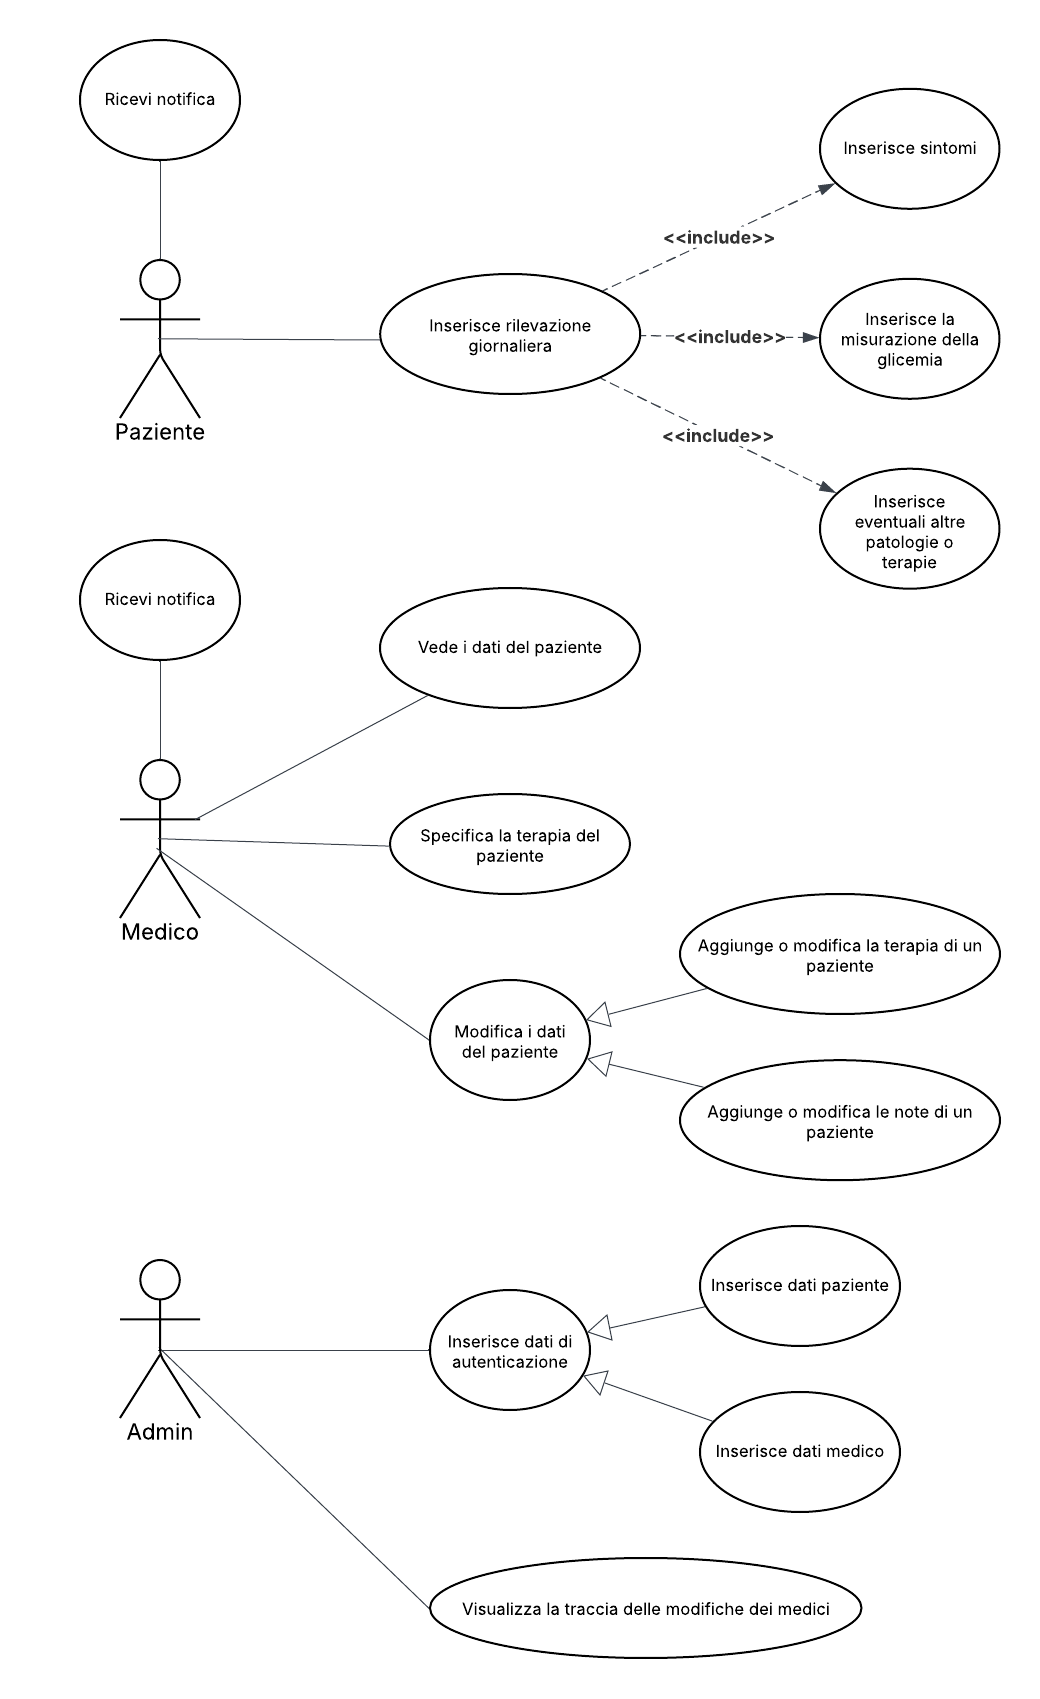
\includegraphics[width=0.7\textwidth]{usecase}
  \caption{Diagramma dei casi d'uso}
  \label{fig:usecase}
\end{figure}

\subsection{Casi d'uso del paziente}

Una volta che il paziente si è autenticato ed è entrato all'interno della sua area riservata, egli può
inserire i dati giornalieri relativi alla sua glicemia (prima e dopo ogni pasto); per fare questo
ha bisogno di inserire dati quali: sintomi, rilevazione glicemica, eventuali altre patologie o terapie.

\subsubsection{Inserimento dei dati giornalieri}

\begin{mdframed}
  \textbf{Attore}: Paziente\\
  \textbf{Precondizioni}: Il paziente deve essere autenticato\\
  \textbf{Passi}: 
  \begin{enumerate}[nosep]
    \item Il paziente accede alla sua home page
    \item Il paziente entra dentro l'area di inserimento dei dati giornalieri
    \item  Il paziente inserisce il dato della sua glicemia prima pasto e dopo pasto
      \begin{itemize}
        \item  Il paziente può aprire un ulteriore finestra per inserire i sintomi, le terapie e le patologie, con oppurtuna data 
        \item  Può anche inserire le assunzioni di insulina o qualsiasi farmaco prescritto dal diabetologo, specificandone giorno, ora, farmaco e quantità assunta
      \end{itemize}
    \item Il paziente inserisce la data e ora di rilevazione
    \item Il paziente conferma l'inserimento dei dati
  \end{enumerate}
  \textbf{Postcondizioni}: La rilevazione è inserita 
\end{mdframed}
\noindent
Andiamo a specificare come viene gestito \textbf{l'inserimento dei dati} del paziente: i dati glicemici sono quelli
che il paziente inserisce giornalmente e obbligatori per inviare le rilevazioni. Dopo aver inserito i dati, l'utente può anche:
\begin{itemize}
  \item inserire specifiche sulla patalogia, terapia o sintomi
  \item inserire le assunzioni di insulina o qualsiasi altro farmo prescritto dal diabetologo
\end{itemize}

\begin{figure}[H]
  \centering
  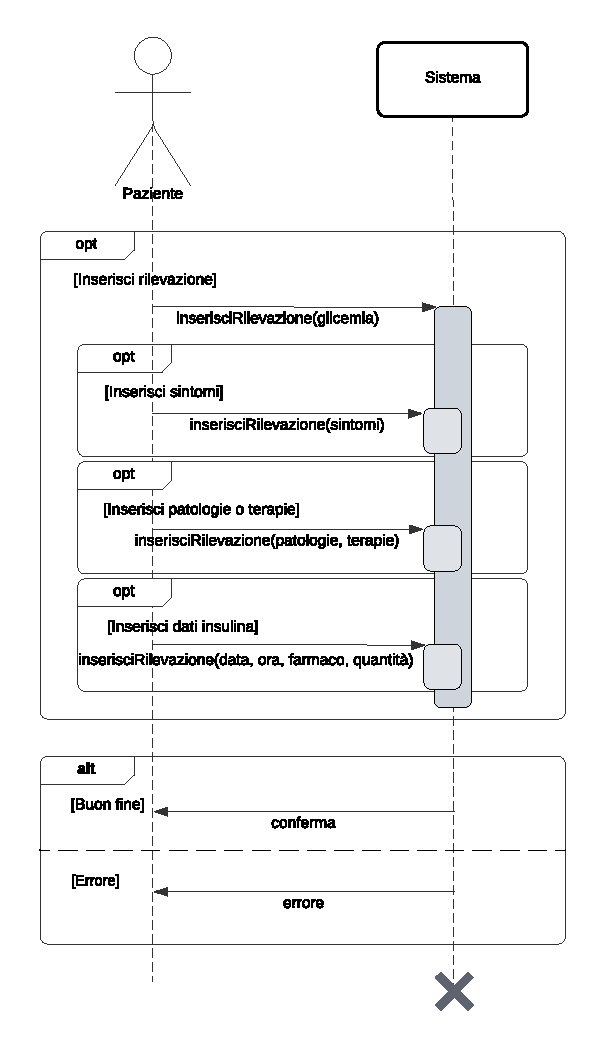
\includegraphics[width=0.7\textwidth]{sdPaziente}
  \caption{Sequence Diagram della rilevazione del paziente}
  \label{fig:sdPaziente}
\end{figure}

\subsection{Casi d'uso del medico}

\subsubsection{Visualizzare i dati del paziente}

\begin{mdframed}
  \textbf{Attore}: Medico\\
  \textbf{Precondizioni}: Il medico deve essere autenticato\\
  \textbf{Passi}: 
  \begin{enumerate}[nosep]
    \item Il medico accede alla sua area riservata
    \item Il medico può accedere alla lista dei pazienti
    \item Il medico può visualizzare i dati del paziente e lo storico delle rilevazioni
  \end{enumerate}
  \textbf{Postcondizioni}: nessuna
\end{mdframed}
\noindent
Il medico una volta che ha acceduto alla sua area riservata può visualizzare i dati di tutti i pazienti. 

\subsubsection{Modificare i dati del paziente}
\begin{mdframed}
  \textbf{Attore}: Medico\\
  \textbf{Precondizioni}: Il medico deve essere autenticato\\
  \textbf{Passi}: 
  \begin{enumerate}[nosep]
    \item Il medico accede alla sua area riservata
    \item Il medico accede alla lista dei pazienti
    \item Il medico seleziona il paziente che vuole gestire
    \item Il medico può decidere tra le seguenti opzioni:
      \begin{itemize}
        \item Aggiungere o modificare la terapia del paziente
        \item Aggiungere o modificare le note di un paziente
      \end{itemize}
    \item Il medico conferma le modifiche
    \item Il sistema aggiorna i dati del paziente
  \end{enumerate}
  \textbf{Postcondizioni}: La modifica è effettuata\\
  \textbf{Sequenza alternativa 1}: il medico può in qualunque momento decidere di annullare le modifiche
  e ritornare alla lista dei pazienti\\
  \textbf{Postcondizioni}: La modifica non è effettuata
\end{mdframed}
\noindent

\begin{figure}[H]
  \centering
  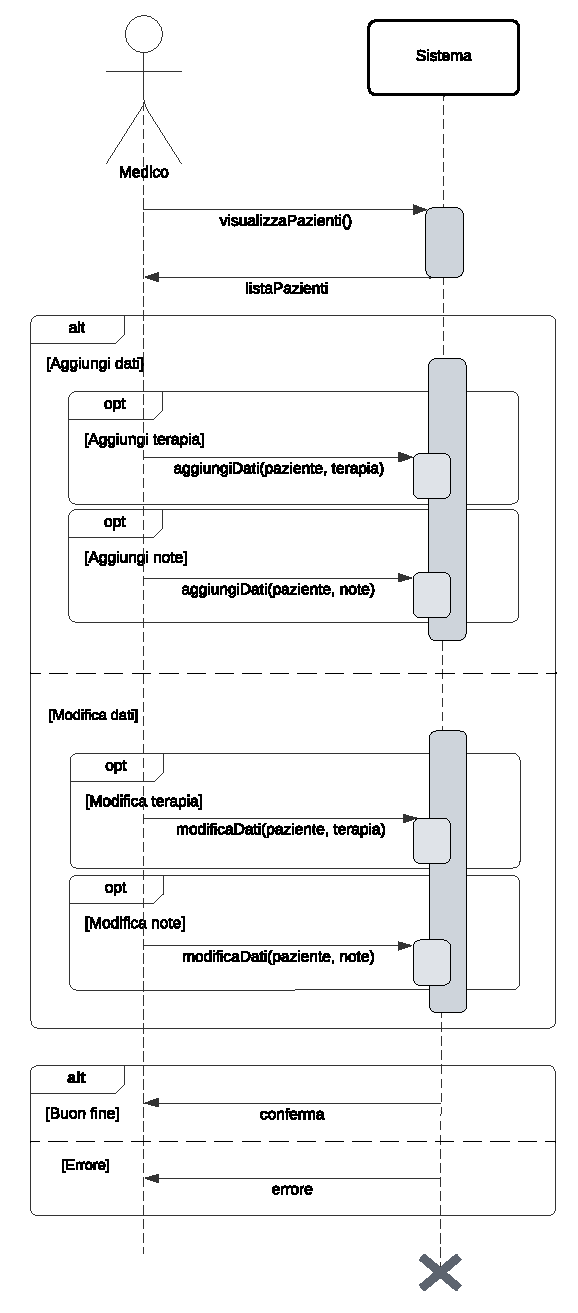
\includegraphics[width=0.65\textwidth]{sdMedico}
  \caption{Sequence Diagram del medico}
  \label{fig:sdMedico}
\end{figure}

\subsection{Ricezione delle notifiche}

Il paziente può ricevere notifiche dal sistema; se il pazienta si dimentica di assumere i farmaci
il sistema può inviare una notifica per ricordarglielo. 

\begin{mdframed}
  \textbf{Attore}: Paziente o Medico\\
  \textbf{Precondizioni}: Il paziente o medico deve essere autenticato\\
  \textbf{Passi}: 
  \begin{enumerate}[nosep]
    \item Il paziente o medico accede alla sua home page
    \item Il paziente o medico entra dentro la sezione delle notifiche
    \item  Il paziente o medico può visualizzare:
      \begin{itemize}
        \item  Notifiche già lette
        \item  Notifiche non lette
      \end{itemize}
  \end{enumerate}
  \textbf{Postcondizioni}: Se viene visualizzata una notifica, questa viene marcata come letta
\end{mdframed}


\begin{figure}[H]
  \centering
  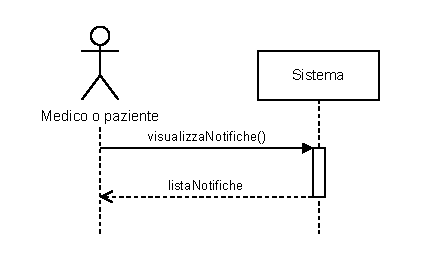
\includegraphics[width=0.7\textwidth]{sdNotifList.pdf}
  \caption{Sequence Diagram della notifica con lista}
  \label{fig:sdNotifList}
\end{figure}
\noindent
Il sistema invia delle notifiche ai seguenti attori:
\begin{itemize}
  \item \textbf{Al paziente}: per ricordargli di inserire i dati giornalieri
  \item \textbf{Al medico di riferimento del paziente}: per avvisare che il paziente  
    non ha seguito per più di tre giorni consecutivi le prescrizioni.
  \item \textbf{A tutti i medici}: per segnalare i pazienti che registrano
    livelli di glicemia sopra le soglie indicate.
\end{itemize}

\subsection{Casi d'uso dell'amministratore}

L'amministratore del servizio può gestire gli utenti del sistema. Si occupa di creare, modificare e cancellare
gli account dei pazienti e dei medici. Per agevolare l'aggiunta di utenti, ci si può registrare
tramite un form di registrazione (che specificherà il ruolo), ma l'amministratore deve comunque
approvare la registrazione per rendere l'utente attivo nel sistema.

\subsubsection{Gestione dell'utente}

\begin{mdframed}
  \textbf{Attore}: Amministratore\\
  \textbf{Precondizioni}: L'amministratore deve essere autenticato\\
  \textbf{Passi}: 
  \begin{enumerate}[nosep]
    \item L'amministratore accede alla sua area riservata
    \item L'amministratore visualizza la lista degli utenti
    \item L'amministratore può:
      \begin{itemize}
        \item  Creare un nuovo utente
        \item  Modificare un utente
        \item  Cancellare un utente
      \end{itemize}
  \end{enumerate}
  \textbf{Postcondizioni}: L'utente è creato, modificato o cancellato
\end{mdframed}

\subsubsection{Gestione delle richieste di registrazione}

\begin{mdframed}
  \textbf{Attore}: Amministratore\\
  \textbf{Precondizioni}: L'amministratore deve essere autenticato\\
  \textbf{Passi}: 
  \begin{enumerate}[nosep]
    \item L'amministratore accede alla sua area riservata
    \item L'amministratore visualizza la lista delle richieste
    \item Seleziona una richiesta di registrazione
    \item L'amministratore può:
      \begin{itemize}
        \item  Accettare una registrazione
        \item  Rifiutare una registrazione
      \end{itemize}
  \end{enumerate}
  \textbf{Postcondizioni}: L'utente è accettato o rifiutato
\end{mdframed}

\subsection{Visualizzazione della traccia dei medici}

Il sistema tiene traccia di ogni cambiamento o modifica che i medici effettuano sui pazienti, per 
ragioni di sicurezza.

\begin{itemize}
  \item L'amministratore può visualizzare questa traccia per verificare 
    che i medici non stiano effettuando operazioni non autorizzate.
  \item Il medico può visualizzare la traccia per verificare le operazioni effettuate
    precedentemente su un paziente da parte di altri medici
\end{itemize}

\begin{mdframed}
  \textbf{Attore}: Amministratore\\
  \textbf{Precondizioni}: L'amministratore deve essere autenticato\\
  \textbf{Passi}: 
  \begin{enumerate}[nosep]
    \item L'amministratore accede alla sua area riservata
    \item L'amministratore accede alla pagina di visualizzazione delle tracce 
  \end{enumerate}
  \textbf{Postcondizioni}: nessuna
\end{mdframed}

\begin{mdframed}
  \textbf{Attore}: Medico\\
  \textbf{Precondizioni}: Il medico deve essere autenticato\\
  \textbf{Passi}: 
  \begin{enumerate}[nosep]
    \item Il medico accede alla sua area riservata
    \item Il medico accede alla pagina di visualizzazione dei pazienti
    \item Il medico seleziona il paziente di cui vuole visualizzare la traccia
    \item Il medico accede alla schermata di visualizzazione della traccia dell'utente
  \end{enumerate}
  \textbf{Postcondizioni}: nessuna
\end{mdframed}


\subsection{Activity diagram}

Per semplicità non verrà rappresentato il fatto di poter ripetere le operazioni più volte,
ma si darà per scontato che l'utente possa tornare indietro e ripetere senza riavviare
il software. Vengono quindi rappresentate soltanto le singole attività di operazione.

Si da inoltre per scontato che per ogni attività (tranne la registrazione) l'utente sia
già autenticato e che non ci siano errori di autenticazione.

\subsubsection{Registrazione di un utente}

\begin{figure}[H]
  \begin{center}
    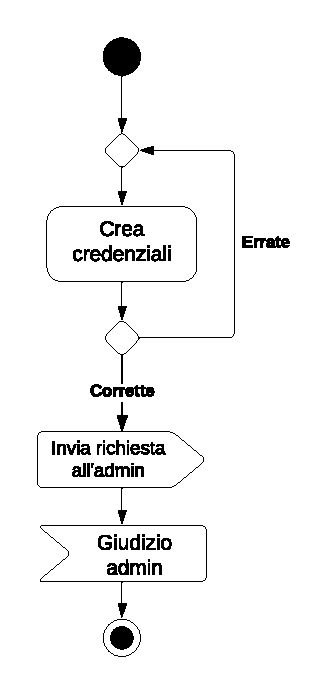
\includegraphics[width=0.4\textwidth]{adRegistrazione}
  \end{center}
  \caption{Activity diagram della registrazione di un utente}
  \label{fig:adRegistrazione}
\end{figure}

\subsubsection{Attività del paziente}

\begin{figure}[H]
  \begin{center}
    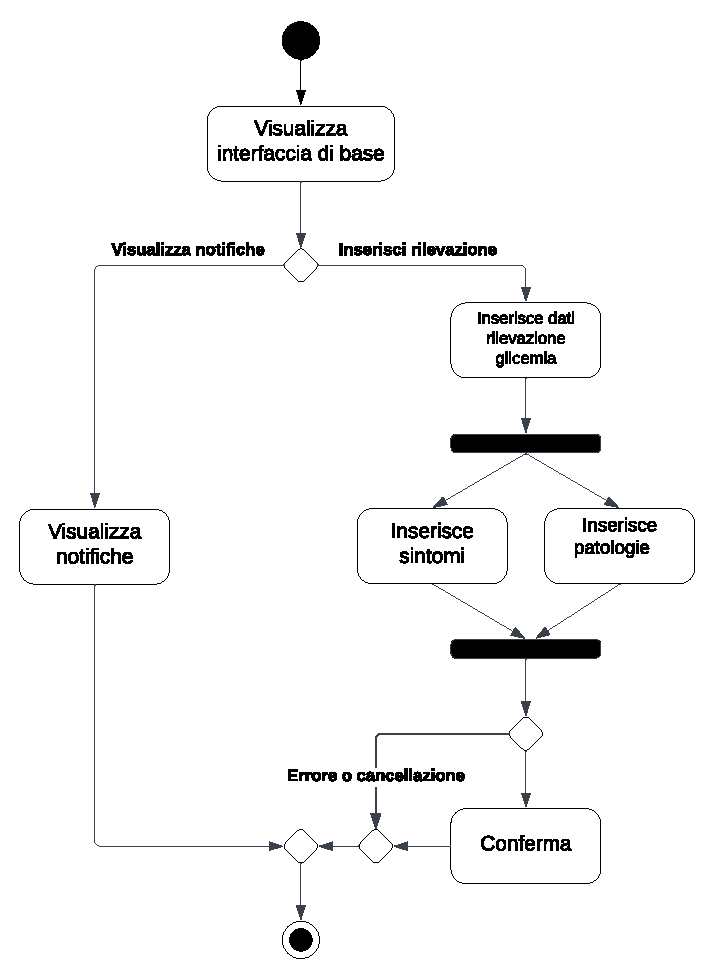
\includegraphics[width=0.8\textwidth]{adPaziente}
  \end{center}
  \caption{Activity diagram del paziente}
  \label{fig:adPaziente}
\end{figure}

\subsubsection{Attività del medico}

\begin{figure}[H]
  \begin{center}
    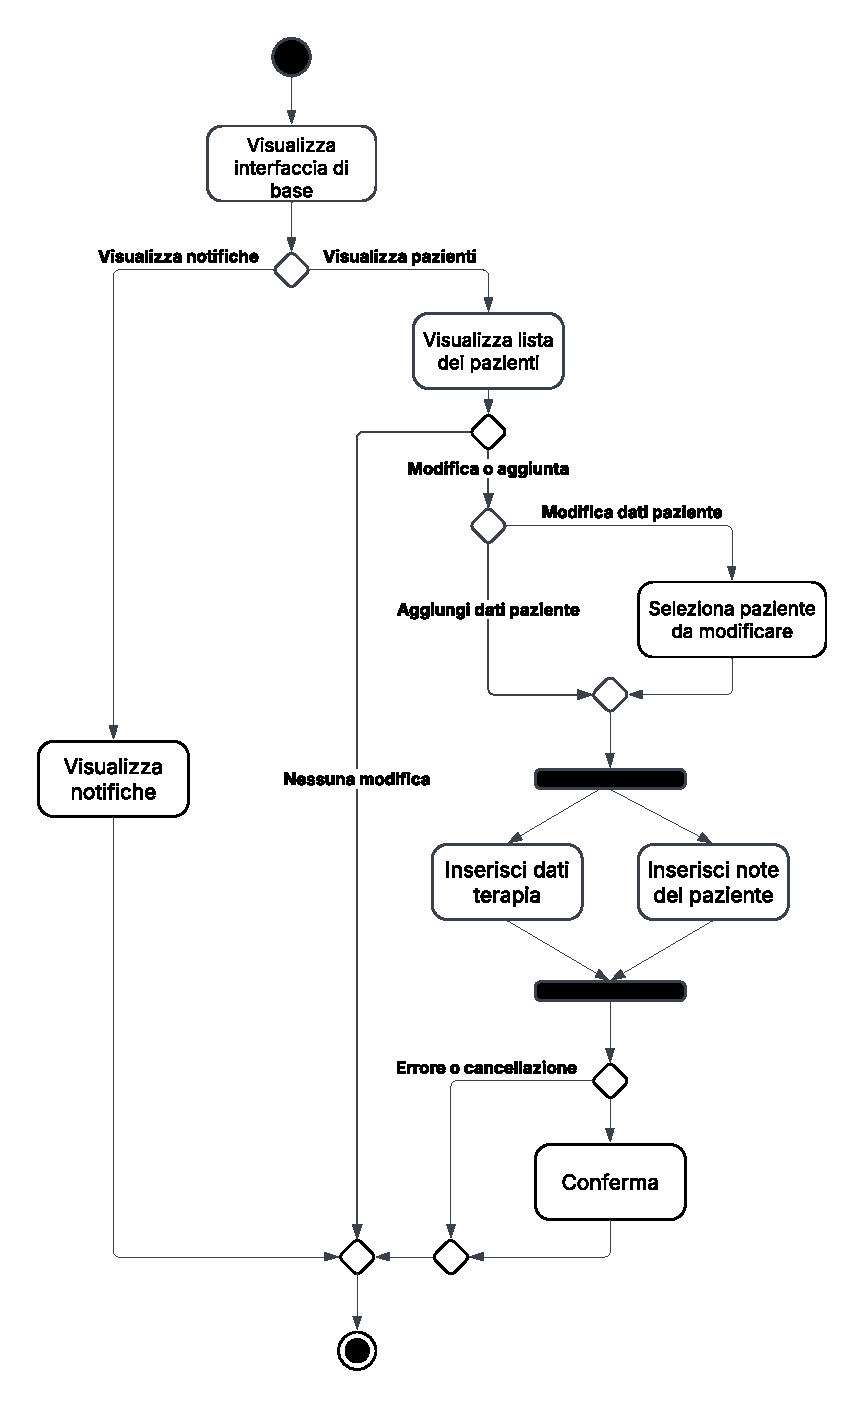
\includegraphics[width=0.9\textwidth]{adMedico}
  \end{center}
  \caption{Activity diagram del medico}
  \label{fig:adMedico}
\end{figure}

\subsubsection{Attività dell'amministratore}

\begin{figure}[H]
  \begin{center}
    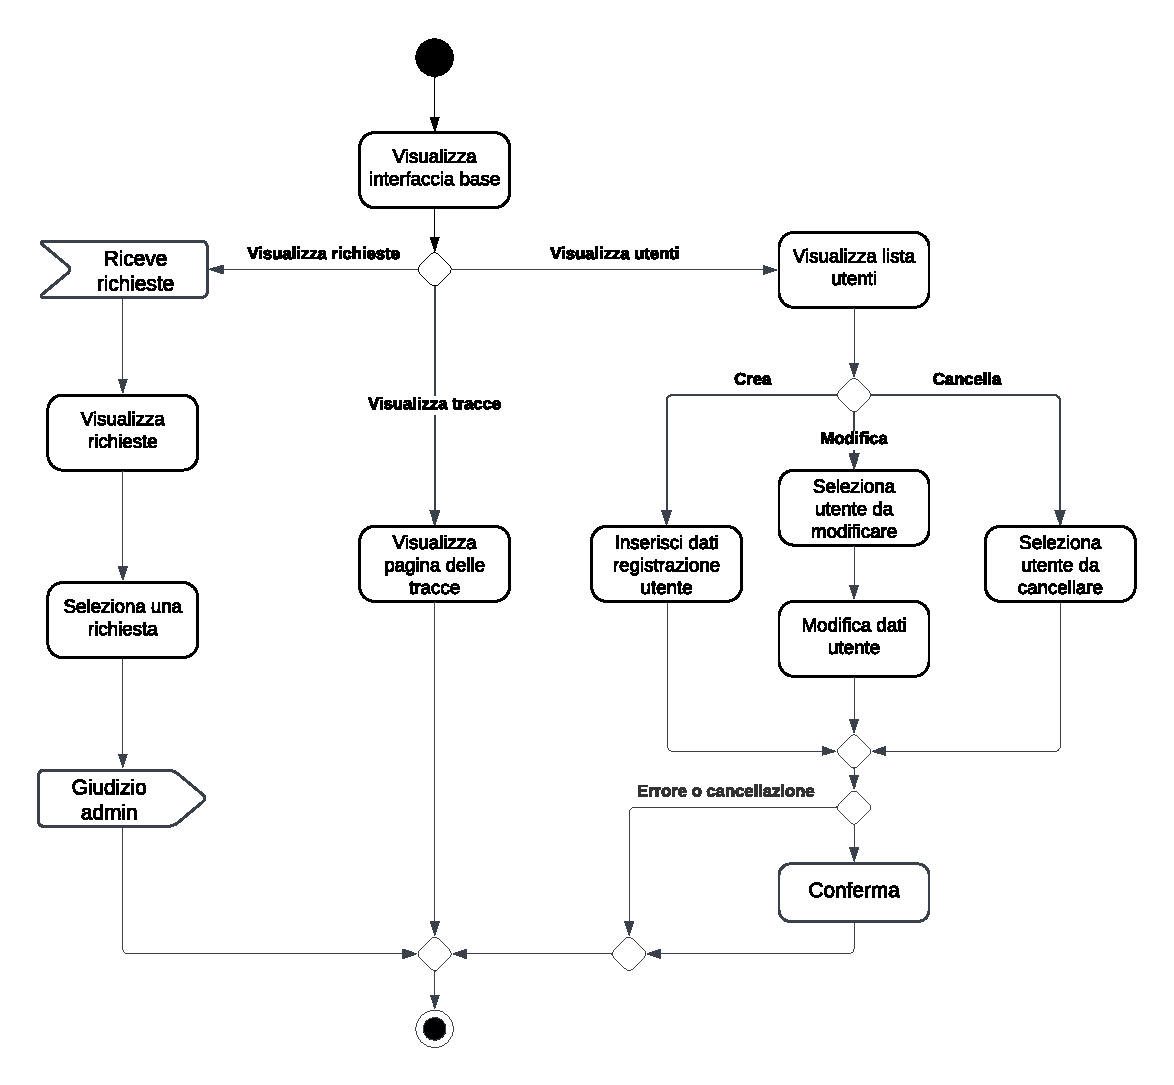
\includegraphics[width=1\textwidth]{adAmministratore}
  \end{center}
  \caption{Activity diagram dell'amministratore}
  \label{fig:adAmministratore}
\end{figure}

\section{Sviluppo}

\subsection{Processo di sviluppo}

Il processo di sviluppo del software è stato realizzato seguendo il modello \textit{Agile} con metodologia \textit{Scrum}.
Il team è composto da due sviluppatori, che hanno lavorato in parallelo su diverse funzionalità del software.
Lo Scrum ci ha permesso di organizzare il lavoro in sprint precisi, durante i quali abbiamo
sviluppato le funzionalità richieste, testandole e integrandole nel software. 
Gli sprint venivano pianificati in base alle funzionalità da implementare e alle priorità stabilite all'inizio,
facendo una scrematura delle funzionalità da implementare in base al tempo a disposizione. 
Alla fine di ogni sprint, abbiamo effettuato una revisione del lavoro svolto, testando le funzionalità implementate e correggendo eventuali bug.
\textit{Product Backlog} e \textit{Sprint Backlog} non sono nient'altro che una lista di "to-do" task che bisogna affrontare per la scelta delle funzionalità da implementare
e su come implementarle rispettivamente. Tuttavia non vi è un \textit{Scrum Master} in quanto il team è composto da due persone e non vi è la necessità di avere una figura che coordini il lavoro.
\begin{figure}[H]
  \begin{center}
    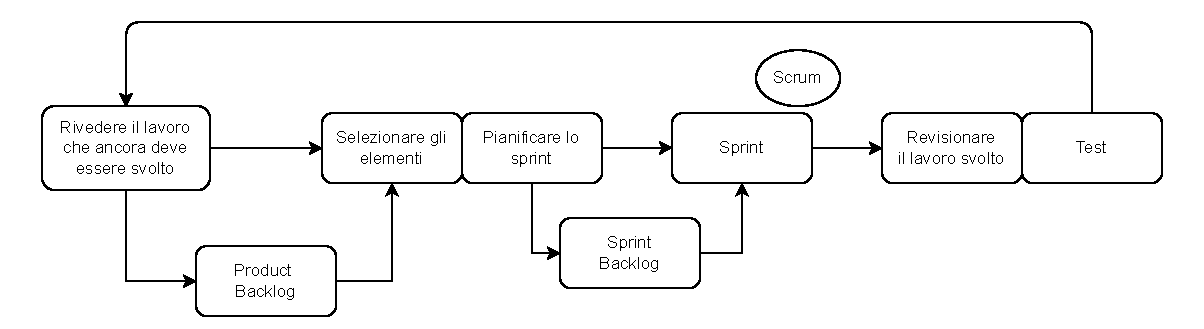
\includegraphics[width=1\textwidth]{adProcessodiSviluppo.pdf}
  \end{center}
  \caption{Diagramma del processo di sviluppo}
  \label{fig:adProcessodiSviluppo}
\end{figure}
\noindent
Prima di cominciare il ciclo di Scrum però, è stata effettuata una fase di \textit{analisi dei requisiti}, dove tutto il team di Scrum si è unito per 
analizzare le specifiche del progetto e poi sono stati definiti i casi d'uso (vedi figura \ref{fig:usecase}).
Man mano che venivano implementate le classi e le funzionalità, venivano costruiti gli UML per rappresentare le classi e le relazioni tra di esse.
Per la gestione del codice sorgente, è stato utilizzato \textit{Git} come sistema di versionamento, con un repository su \textit{GitHub} per facilitare la collaborazione tra i membri del team.
Abbiamo utilizzato anche \textit{Github Planner} per tenere traccia delle attività da svolgere e dello stato di avanzamento del progetto.

\begin{figure}[H]
  \begin{center}
    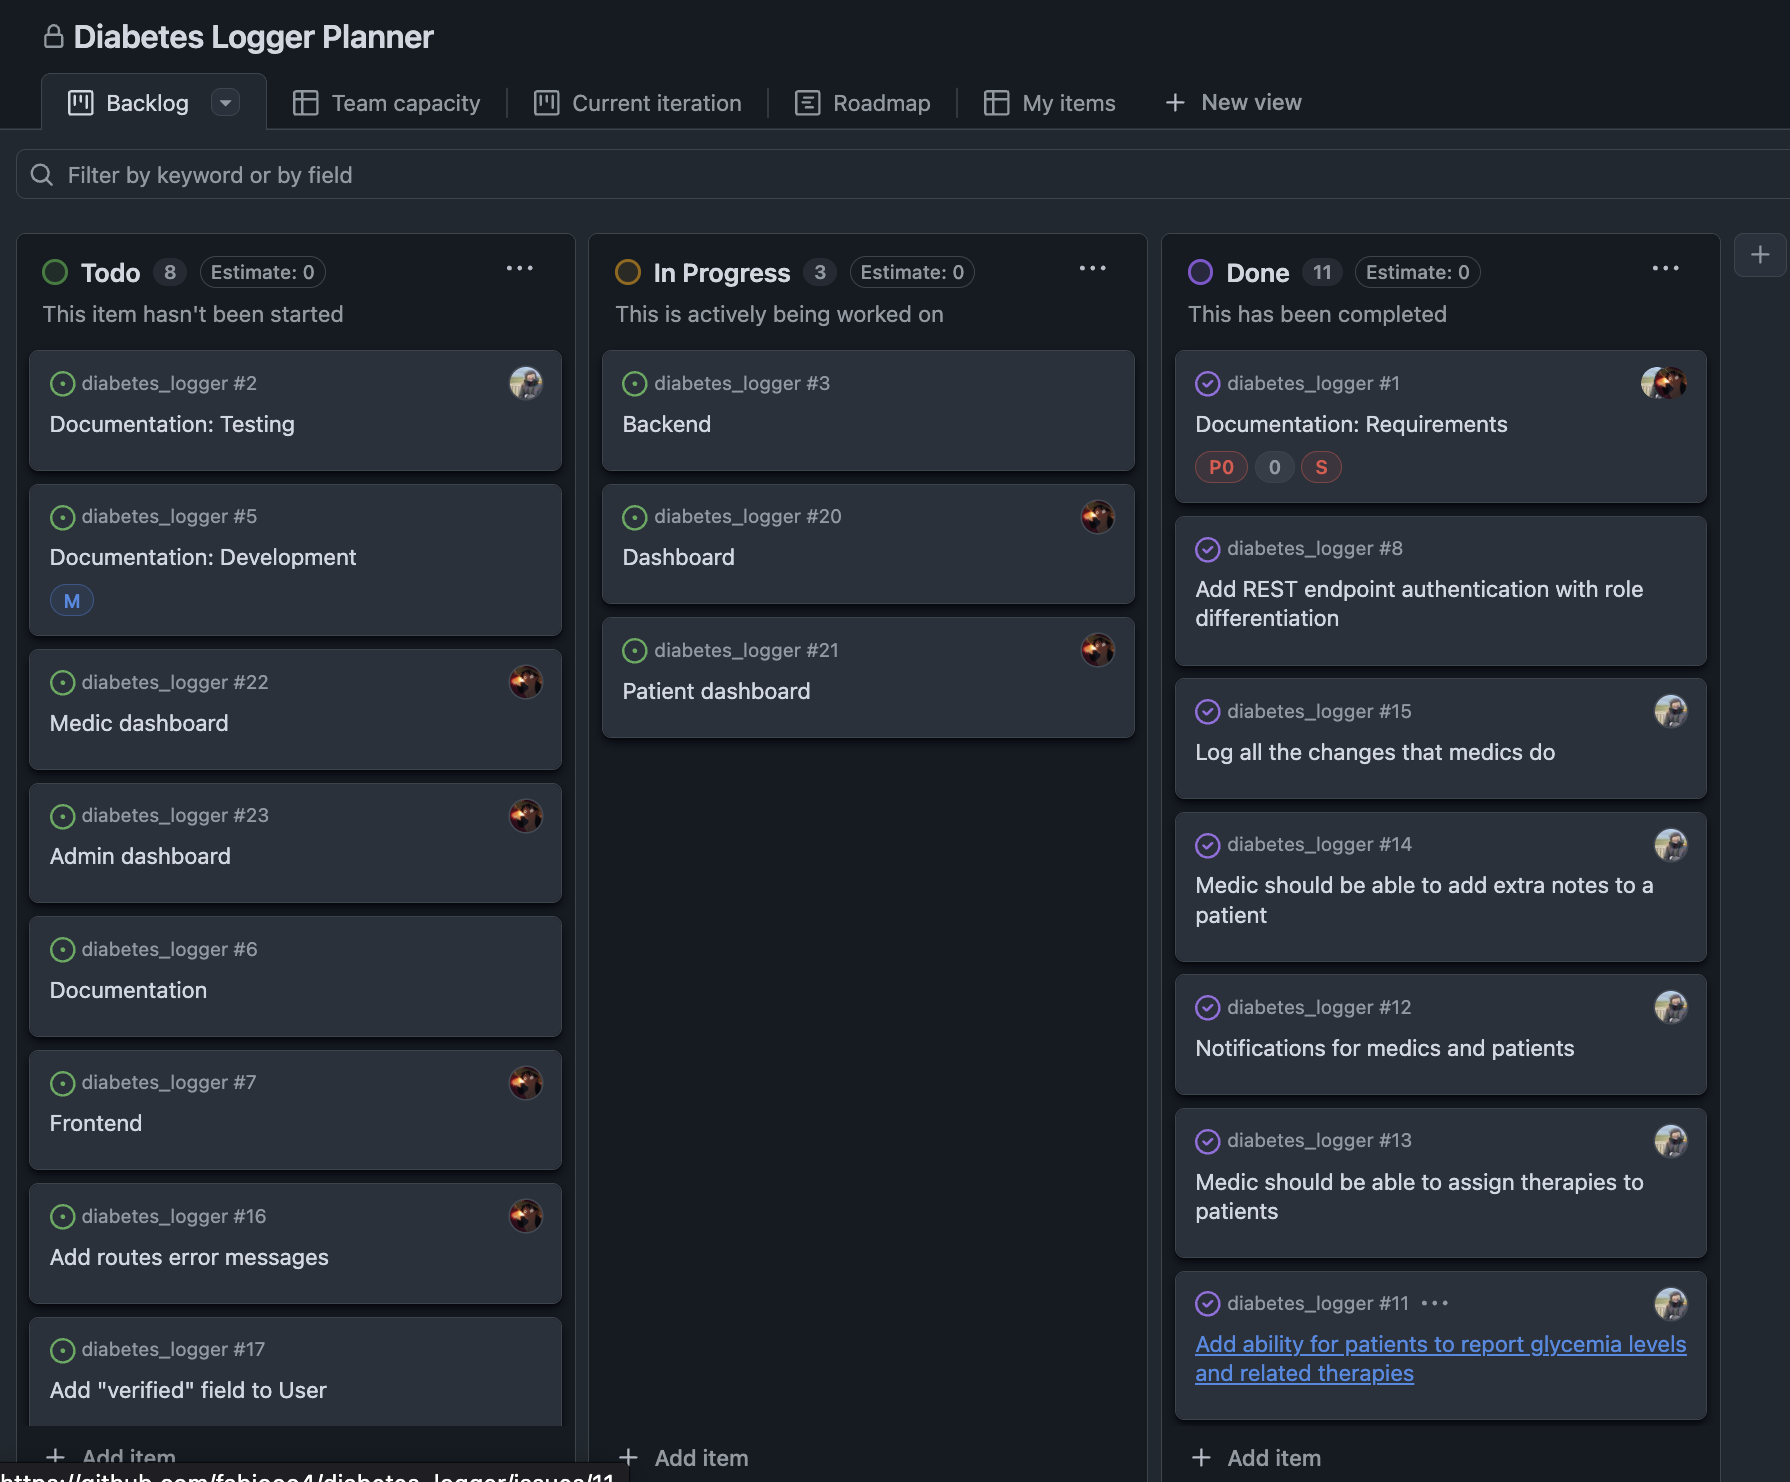
\includegraphics[width=0.9\textwidth]{githubPlanner.png}
  \end{center}
  \caption{Github Planner del progetto} 
  \label{fig:githubPlanner}
\end{figure}

\subsection{Progettazione e pattern architetturali usati}

Il software è stato progettato seguendo il pattern architetturale \textit{Model-View-Controller} 
(MVC), che separa la logica di business, la presentazione e la gestione degli eventi.
Questo tipo di pattern ci ha permesso di mantenere il codice ben organizzato e facilmente manutenibile.
Abbiamo scelto questo pattern poiché \textit{Spring Boot} (framework di Java utilizzato per il backend) ha gli strumenti necessari
per implementare questo pattern in modo semplice e veloce:
\begin{itemize}
  \item \textbf{Model}: rappresenta la logica di business e i dati del software. 
  In questo caso, il model è composto da classi che rappresentano lo user, i pazienti, i medici, 
  le rilevazioni, le notifiche e il change log. 
  \item \textbf{View}: rappresenta la parte di presentazione del software. In questo caso, 
  la view è composta da pagine costruite con SvelteKit, un framework per fare siti web. 
  \item \textbf{Controller}: rappresenta la parte di gestione degli eventi e della logica di business. 
  Risponde alle chiamate e alle sollecitazioni della View e gestisce le richieste degli utenti.
\end{itemize}
Tramite richieste HTTP, il controllera comunica con il model e la view. 
Quindi il controller riceve la richiesta dalla view e poi interagisce con il model per 
ottenere i dati necessari oppure modificarli in base alla richiesta dell'utente.
Nelle prossime sezioni verrà analizzato in dettaglio il modello Model poiché contiene 
le classi che rappresentano gli attori del sistema e le loro interazioni.

\begin{figure}[H]
  \begin{center}
    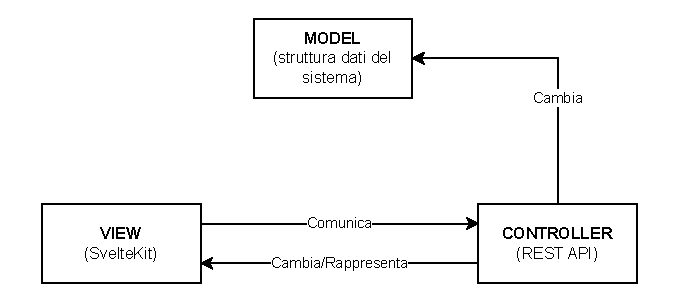
\includegraphics[width=0.9\textwidth]{MVC.pdf}
  \end{center}
  \caption{Architettura MVC del software} 
  \label{fig:mvc}
\end{figure}




\end{document}
